\documentclass[10pt]{article}

\usepackage[margin=0.82in]{geometry}
\usepackage{amsmath,amssymb}
\usepackage{booktabs}
\usepackage{graphicx}
\usepackage[hypertexnames=false]{hyperref}
\usepackage{enumitem}
\usepackage{float}
\usepackage{xurl}

\graphicspath{{docs/}{./}}
\title{HyperNPA: Held-Out Evaluation of Image-Conditioned Neural Particle Automata}
\author{burn\_automata Research Notes}
\date{July 10, 2026}

\newcommand{\npa}{\mathrm{NPA}}

\begin{document}
\maketitle

\begin{abstract}
HyperNPA studies amortized generation of Neural Particle Automata (NPA) from
images. A frozen DINOv2 ViT-S/14 encoder produces spatial condition tokens; a
deterministic hypernetwork emits a LoRA adapter for a shared growing NPA; and
the adapted NPA is optimized through differentiable particle rollout and an
alpha-aware image objective. This revision corrects an earlier teacher-leakage
interpretation and reports identity-disjoint validation.

The strongest teacher-free catalog result reaches 10.52 dB aggregate
composited PSNR at 4096 particles and 1024 rollout steps. On an OmniSVG-1k
split with 900 train and 100 held-out images, patch RGB channels and local
condition control raise selected aggregate PSNR from 11.35 to 11.76 dB, but
remain far below the 26 dB target. A direct 1000-row adapter table reaches only
12.35 dB even on its training identities. Unfreezing the shared trunk lowers
the short-rollout objective while degrading long-rollout PSNR; a longer
512-particle, 32--64-step curriculum improves p10 PSNR from 10.49 to 10.80 dB
without improving aggregate PSNR. These controls locate the present bottleneck
in the shared-basis and rollout-training objective, before amortized DINO
conditioning or stochastic adapter flow.
\end{abstract}

\section{Architecture}

For condition image $c$, shared NPA parameters $W$, and generated adapter
$a_\phi(c)$, the maintained deterministic path is
\[
c \xrightarrow{\text{DINOv2}} z_c
\xrightarrow{h_\phi} a_\phi(c), \qquad
x_{t+1},s_{t+1}=\npa_{W,a_\phi(c)}(x_t,s_t).
\]
The loss is evaluated on Gaussian particle splats and combines target color,
density, composited RGB, displacement, overflow, and boundary terms.

\paragraph{Condition tokens.}
Inputs are resized to the native 224-pixel DINO ViT-S/14 resolution. The CLS
token and $16\times16$ patch grid produce 257 tokens with 384 DINO channels.
Alpha-aware runs append patch occupancy, yielding $257\times385$. The latest
ablation also appends patch-aligned RGB, yielding $257\times388$. DINO inference
runs on GPU without an autodiff graph, in bounded batches or a bounded resident
device cache.

\paragraph{Adapter generator.}
The current scaling path uses a module-aware cross-attention decoder and emits
a rank-82 LoRA adapter. Rank 82 is sufficient to represent the released
growing-NPA matrix deltas exactly. The artifact name retained from earlier work
contains \texttt{rectified\_flow}, but the maintained one-step generator is
deterministic. It is not a stochastic flow model.

\paragraph{Spatial control.}
An optional per-step field samples patch-token features at particle positions
and adds a learned local residual. A state-aware extension also projects the
current recurrent state into that controller. Its projection is initialized to
zero, preserving the previous checkpoint exactly before training. Per-step
field artifacts cannot be collapsed to static LoRA-only NPA artifacts and are
therefore rejected by the static Bevy inference path.

\section{Evaluation Protocol}

Teacher adapters are attached only to training examples. The trainer aborts if
any holdout example contains an oracle adapter target. Quality reports include
composited, raw-render, foreground, and density PSNR; density soft IoU;
generated-over-base and correct-over-shuffled gaps; adapter diagnostics; and an
optional nearest-training-oracle control.

The catalog quality protocol uses official transparent targets, 4096 particles,
1024 rollout steps, update probability 0.5, and seed 42. OmniSVG-1k uses a
deterministic 900/100 identity split and reports 1024-particle, 128-step quality
on a fixed 16-image holdout subset. Checkpoint selection uses p10 composited
PSNR to prevent aggregate improvements from hiding tail regressions.

\section{Released-Catalog Controls}

An earlier two-image result reconstructed the exact rose and tropical-fish
adapter targets and reached 27.57 dB aggregate composited PSNR. Because those
adapters were included in training, this proves adapter materialization and
runtime correctness, not held-out image-to-NPA generalization.

The corrected split trains on eight released identities and holds out rose and
tropical fish without teacher adapters.

\begin{table}[H]
\centering
\small
\begin{tabular}{lr}
\toprule
strict 8/2 catalog metric & result \\
\midrule
aggregate composited RGB PSNR & 10.52 dB \\
p10 composited RGB PSNR & 9.83 dB \\
mean raw-render RGB PSNR & 11.21 dB \\
aggregate density PSNR & 8.11 dB \\
mean density soft IoU & 0.498 \\
correct condition over shuffled & 0.09 dB \\
generated adapter over shared base & 2.33 dB \\
nearest-training DINO oracle adapter & 8.90 dB \\
\bottomrule
\end{tabular}
\caption{Teacher-free catalog holdout quality at 4096 particles and 1024
steps. The nearest-oracle result is lower than the generated adapter and does
not provide a path to parity.}
\label{tab:catalog-heldout}
\end{table}

\section{OmniSVG-1k Ablations}

\begin{table}[H]
\centering
\scriptsize
\resizebox{\linewidth}{!}{%
\begin{tabular}{lrrr}
\toprule
experiment & aggregate composited PSNR & p10 PSNR & median training throughput \\
\midrule
static DINO+alpha module decoder & 11.35 dB & 8.82 dB & 1.11M particle-steps/s \\
append patch RGB channels & 11.53 dB & 9.21 dB & 1.10M particle-steps/s \\
add per-step spatial output control & 11.76 dB & 9.34 dB & 1.00M particle-steps/s \\
add recurrent-state control & 11.76 dB selected & 9.34 dB selected & 0.92M particle-steps/s \\
direct sample-ID adapter table (train upper bound) & 12.35 dB & 10.49 dB & 1.92M particle-steps/s \\
adapter table, 512p / 32--64-step curriculum & 12.30 dB & 10.80 dB & 0.59M particle-steps/s \\
\bottomrule
\end{tabular}}
\caption{Identity-disjoint HyperNPA ablations and non-amortized train upper
bounds. The adapter-table rows evaluate training identities and therefore are
ceilings, not held-out generalization results.}
\label{tab:omnisvg-ablation}
\end{table}

Patch RGB improves the aggregate by 0.18 dB and the p10 tail by 0.39 dB. Local
output control adds another 0.23 dB aggregate. State-aware control improves the
short objective and a later aggregate checkpoint, but lowers the p10 selection
score, so the state-independent checkpoint remains selected.

The sample-ID table removes DINO and adapter prediction entirely. Its 12.35 dB
train ceiling is the central diagnostic result: the current shared basis and
rollout optimization cannot fit the 1k training set near oracle quality. A
5000-step short-rollout continuation adds only 0.21 dB. Updating the shared
trunk lowers sampled loss from roughly 3.0 to 2.59 while long-horizon PSNR
regresses, demonstrating objective mismatch. The longer curriculum improves
the p10 tail by 0.31 dB but not the aggregate.

This upper bound is specific to the tested curriculum, not an intrinsic LoRA
expressivity result. The released growing trainer uses 4096 particles, 32--96
sampled rollout steps, a 256-pixel splat grid, 4096 target points, a 512-state
pool, batch size 8, seed injection every 16 epochs, brush damage 0.1, and three
10k-epoch repetitions. Our 1k controls use 256/512 particles, 8--64 steps, a
64-pixel loss grid, 2048 target points, two pool slots per identity, and only
hundreds of visits per identity. The next experiment therefore depends on a
sparse/tiled 4096-particle Burn backward path capable of reproducing the
upstream regime.

\section{Renderer Evidence}

\begin{figure}[p]
\centering
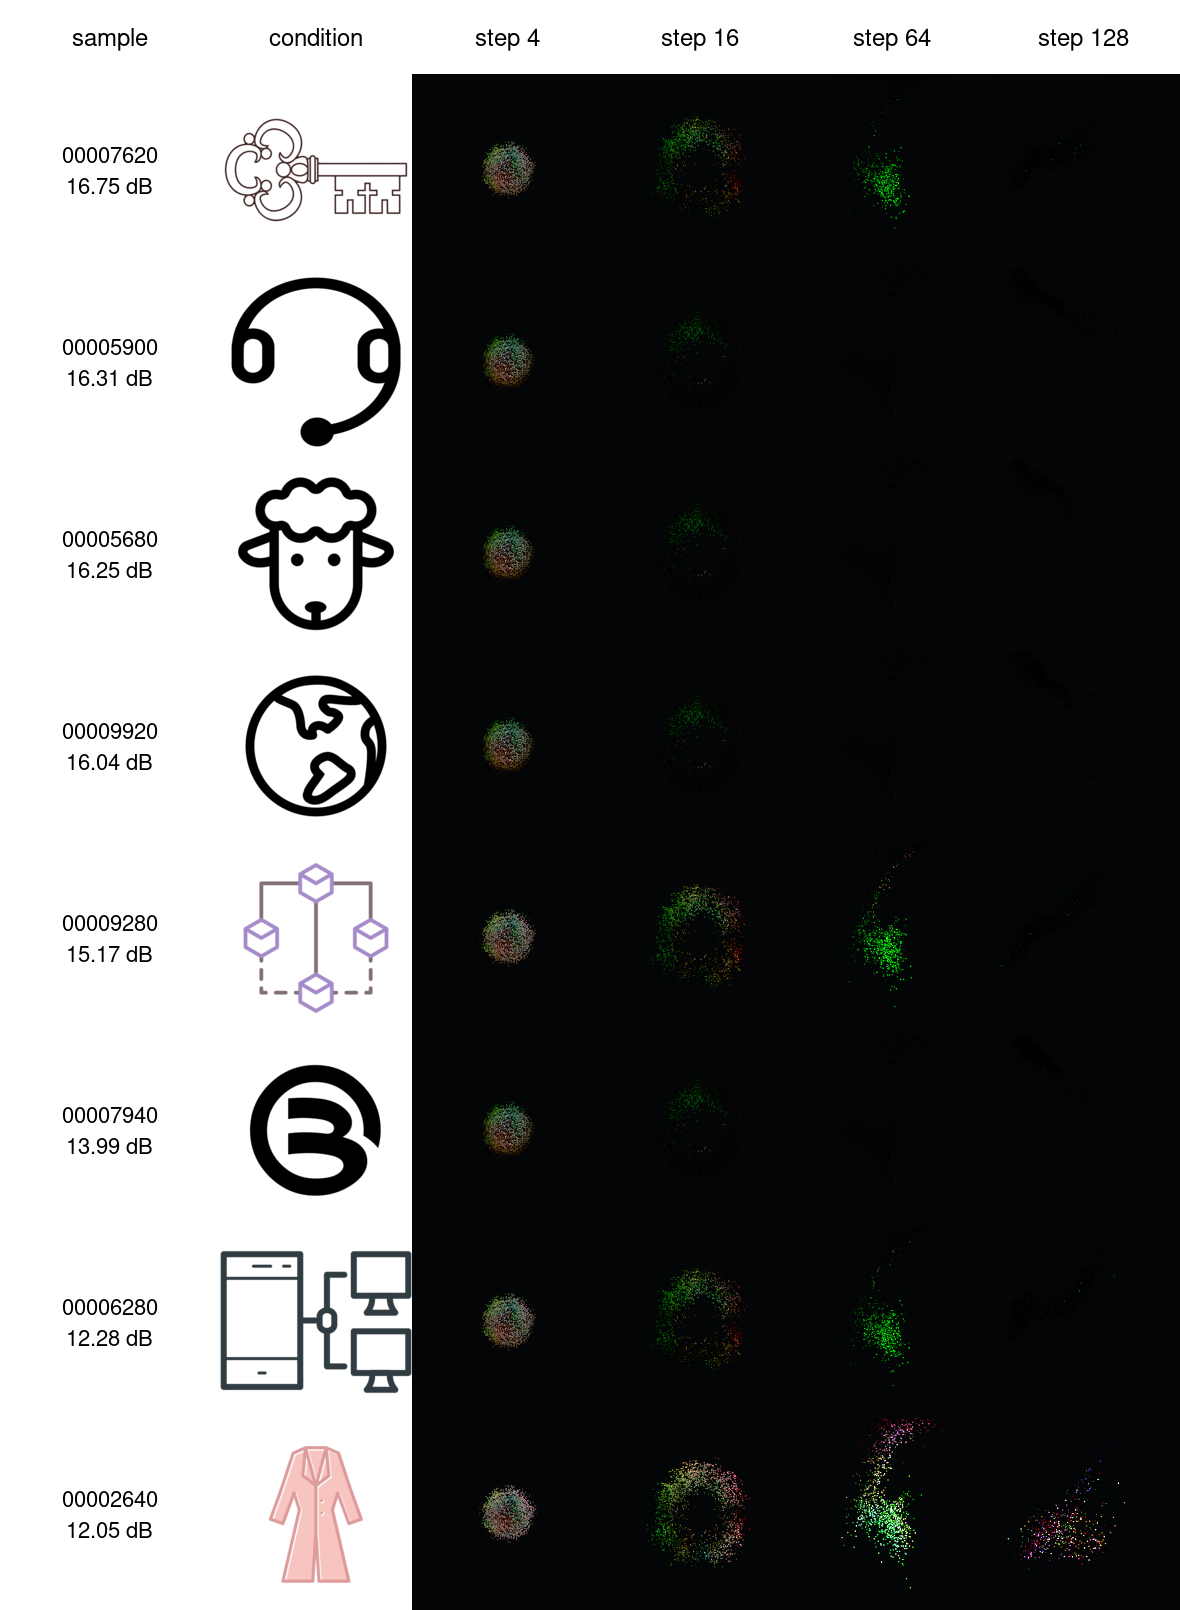
\includegraphics[height=0.72\textheight,keepaspectratio]{hyper_npa_figures/e2e_bevy_rollouts/e2e_hypernpa_bevy_rollout_panel.png}
\caption{Actual Bevy/WGPU and \texttt{bevy\_gaussian\_splatting} captures from
eight held-out conditions at multiple rollout steps. This panel is retained as
an inference-integration and failure-mode record from an earlier 10k
checkpoint; it is not used for the strict numerical claims in
Tables~\ref{tab:catalog-heldout} and~\ref{tab:omnisvg-ablation}. Sparse and
collapsing late rollouts illustrate the quality gap.}
\label{fig:bevy-rollouts}
\end{figure}

\section{Discussion}

The experiments reject four simple explanations for the gap. First, holdout
DINO tokens are available and condition shuffling changes outputs on OmniSVG.
Second, explicit RGB information helps but is not sufficient. Third, a larger
local controller lowers training loss but does not solve the tail. Fourth,
direct adapters without a hypernetwork are themselves far below oracle
quality. The first unresolved problem is therefore learning a robust shared NPA
basis under a quality-scale recurrent objective.

The next gate is:
\begin{enumerate}[leftmargin=*]
  \item train shared-trunk plus direct adapters at particle counts and rollout
  horizons overlapping validation;
  \item compare each row to an independently overfit NPA oracle with identical
  targets, seeds, particles, and rollout steps;
  \item select on aggregate and p10 oracle-relative quality, never short loss
  alone;
  \item freeze the proven trunk and amortize the direct adapters with DINO
  tokens plus downstream rollout loss;
  \item only then introduce noisy adapter states and timestep-conditioned
  velocity training for a true rectified-flow generator.
\end{enumerate}

\section{Conclusion}

The Burn/WGPU implementation now provides a leakage-safe, identity-disjoint,
GPU-native HyperNPA evaluation stack. It proves conditional control and useful
incremental gains from spatial RGB and local rollout conditioning. It does not
prove generalized oracle-quality image-to-NPA generation: the best strict
held-out scores remain 14--16 dB below the 26 dB target, and the direct-adapter
upper bound is also low. Future claims must first establish a quality-scale
shared NPA basis and then demonstrate that DINO-conditioned amortization retains
that oracle-relative quality.

\begin{thebibliography}{9}
\bibitem{npa}
Self-Organising Neural Particle Automata.
\url{https://selforg-npa.github.io/}
\end{thebibliography}

\end{document}
